\subsubsubsubsection{District stopper}
\begin{figure}[h]
\centering
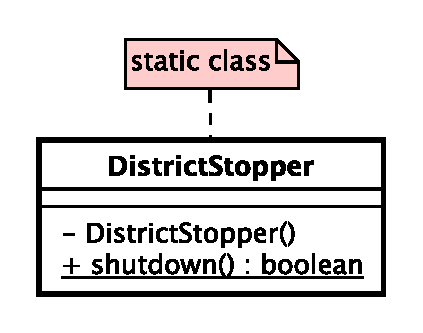
\includegraphics[scale=0.6,keepaspectratio]{images/solution/app/backend/district_stopper.eps}
\caption{\pReactive::DistrictStopper}
\label{fig:sd-app-district-stopper}
\end{figure}
\FloatBarrier
\begin{itemize}
  \item \textbf{\descr} \\
  It has the responsibility to shutdown the application layer.
  It is a static class because it is composed of only static methods.
  \item \textbf{\ops}
  \begin{itemize}
    \item \texttt{DistrictStopper()} \\
    Private and unique constructor because the class provides only static methods 
    so there are no reasons a client creates instances of it.
    \item[+] \texttt{\underline{shutdown() : boolean}} \\
    Terminates the district. Returns true if the process completes neatly,
    false otherwise.
  \end{itemize}
\end{itemize} 
